\section{Effet photoélectrique et lumière}

\subsubsection*{Théorie quantique}
%\subsubsection*{Pages 222 à 236 du livre}

Nous savons à présent que la lumière visible est une onde
électromagnétique, due à des oscillations de charges électriques à des
fréquences comprises entre $4 10^{14} \siunit{Hz}$ et
$8 10^{14} \siunit{Hz} $
(voir spectre électromagnétique).

\subsubsection{Production de la lumière}

\emph{Quelles sont ces charges oscillantes responsables de l'émission de
lumière~?}

\begin{figure}
\centering
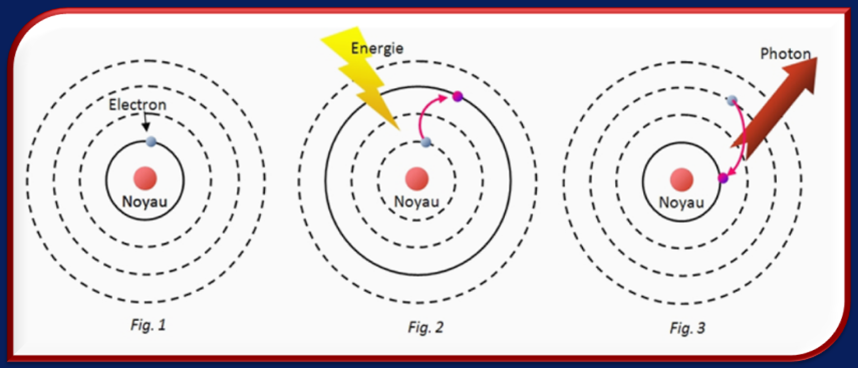
\includegraphics[width=11.557cm,height=4.957cm]{Pictures/100000010000035A00000170D87D5DDA82610A97.png}
\caption{}
\end{figure}

L'émission de lumière par un atome ou une molécule est un
\textbf{phénomène électronique},
provoqué par l'oscillation des électrons atomiques.

Dans un atome chaque électron se trouve sur une orbitale et donc possède
des niveaux d'énergie quantifiés (les niveaux d'énergie ont des valeurs
précises). C'est le modèle de Bohr (fig. 1).

De l'énergie incidente sur la surface d'un objet excite certains
électrons des atomes. L'électron peut passer d'un niveau inférieur vers
un niveau d'énergie plus élevée en absorbant cette énergie (fig. 2). On
parlera d'absorption.

Ces électrons excités retournent très rapidement à un état stable en
perdant l'énergie accumulée sous forme de rayonnement qui est une onde
électromagnétique à savoir un «~paquet d'énergie~électromagnétique~» ou
photon (fig. 3). On parlera d'émission.

Le rayonnement émis peut-être situé dans le visible, mais aussi dans
l\textbf{\textbf{'}\textbf{infrarouge} }ou\textbf{
}l\textbf{\textbf{'ultraviolet}, }tout dépend de la différence d'énergie
entre les deux niveaux lors de la transition électronique.

L'énergie incidente peut provenir~:

\begin{itemize}

\item
  de matériaux chauffés.
\item
  d'un courant électrique appliqué entre des électrodes placées à chaque
  extrémité d'un tube (tube néon).
\end{itemize}

Chaque atome émet une couleur qui lui est propre car la répartition
électronique en couches (modèle de Bohr) est caractéristique de chaque
élément du tableau périodique.

\begin{figure}
\centering
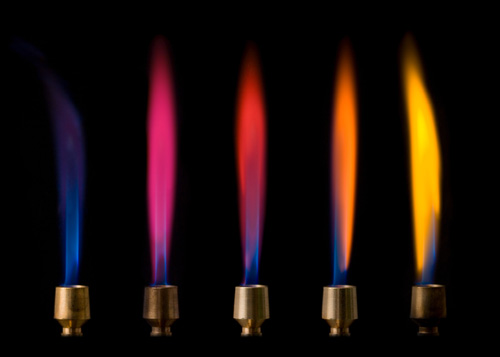
\includegraphics[width=5.856cm,height=4.186cm]{Pictures/10000000000001F4000001658D0506E7D72323B2.jpg}
\caption{}
\end{figure}
\subsubsection{Interaction lumière-matière - l'effet photoélectrique}

C'est 1887, à l'occasion de ses recherches pour prouver l'existence des
ondes électromagnétiques, que le physicien allemand Hertz mis en
évidence l'effet photoélectrique.

Dans cet effet, \textbf{de la lumière qui arrive sur un métal provoque
l'éjection d'électrons présents dans le métal~: il s'agit de l'effet
photoélectrique. }

C'est le principe de fonctionnement des cellules photoélectriques.

\begin{figure}
\centering
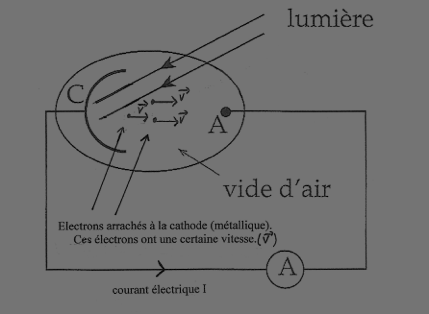
\includegraphics[width=6.638cm,height=4.852cm]{Pictures/10000001000001AD0000013AB85194CC89C1758C.png}
\caption{}
\end{figure}

\subsubsection{La cellule photoélectrique }

De la lumière (de fréquence f ) arrive sur un métal (la cathode C) et
provoque l'éjection d'électrons présents dans le métal. Ces électrons
animés d'une vitesse

\includegraphics[width=0.331cm,height=0.401cm]{Pictures/10000001000000090000000BEA16D6AB6A907BC0.png}
vont produire un courant électrique dans le circuit.

(Rappel~: le sens conventionnel du courant est de sens opposé au sens de
déplacement des électrons).

\subsubsection{Propriétés de l'effet photoélectrique. }

On conçoit bien que la lumière, onde électromagnétique, puisse interagir
avec la surface du métal en y faisant vibrer les électrons peu liés pour
finalement en arracher.

\emph{a) Influence de l'intensité de la lumière :}

L'intensité du courant électrique mesuré (et donc l'effet
photoélectrique) est d'autant plus grand que l'intensité de la lumière
incidente est grande. (L'intensité lumineuse est l'énergie reçue par
unité de surface et par unité de temps. Elle se mesure en
W/m\textsuperscript{2}.)

Eclairer plus intensément correspond à envoyer davantage d'énergie vers
la surface du métal et permet logiquement d'augmenter l'intensité du
courant électrique.

\emph{b) Influence de la nature du métal :}

Chaque métal présente une force de cohésion caractéristique du métal et
l'énergie nécessaire pour arracher un électron dépend logiquement du
métal en présence.

\emph{c) Influence de la fréquence de la lumière :}

Pour chaque métal éclairé, il existe une fréquence de seuil
(f\textsubscript{0}) en dessous de laquelle l'effet photoélectrique ne
se produit pas, \textbf{quelle que soit l'intensité lumineuse, même très
intense.}

Le modèle ondulatoire de la lumière ne permet pas d'expliquer cela.
\subsubsection{Hypothèse du photon d'Einstein. }

Albert Einstein proposa en 1905 une hypothèse révolutionnaire pour
expliquer l'effet photoélectrique.

Selon Einstein, l'énergie lumineuse n'atteint pas une surface de manière
continue, c'est-à-dire à tout moment et partout sur la surface (comme le
prévoit le modèle ondulatoire) mais est cédée à la surface de manière
discontinue, tant du point de vue spatial (au même instant, l'énergie
n'arrive pas partout) que du point de vue temporel (en un point donné,
l`énergie n'arrive qu'à certains instants).

L'absorption de l'énergie lumineuse par une surface peut être comparée à
l'arrivée de projectiles. Elle ne peut se faire que par quantités
indivisibles, appelées quanta ou encore photons.

L'énergie lumineuse transférée à la matière est toujours celle d'un
nombre entier de photon. On dit que cette énergie est quantifiée (on
parlera de la théorie quantique).

Cette énergie dépend de la fréquence comme le montre l'effet
photoélectrique.

\subsubsection{Explication de l'effet photoélectrique~:} lors de
l'interaction lumière-matière, lorsque la lumière atteint la plaque
métallique~:

\begin{itemize}

\item  \textbf{un photon} cède toute son énergie à \textbf{un électron}. Le
  photon, quanta d'énergie («~paquet d'énergie~»), est complètement
  absorbé et disparaît.
\item  Un électron ne peut pas accumuler l'énergie de plusieurs photons.
\item  Pour arracher un électron de la plaque métallique, il faut lui
  communiquer au minimum une énergie W appelée travail d'extraction
  (énergie nécessaire pour rompre la liaison).
\end{itemize}

\subsubsection*{Conclusion}

\begin{itemize}

\item  si $h f < W$ (si l'énergie d'un photon est inférieure au travail
  d'extraction), l'énergie communiquée à l'électron est insuffisante,
  même si beaucoup de photons arrivent et aucun électron ne sera
  arraché. Ceci explique l'existence de la fréquence seuil.
\item  Si $h f > W$ , des électrons sont éjectés de la surface métallique. Une
  partie de l'énergie hf est utilisée pour arracher l'électron hors du
  métal~; l'excédent d'énergie est emporté par l'électron sous forme
  d'énergie cinétique (Ec).
\item Le principe de conservation d'énergie nous permet d'écrire~:
\end{itemize}

L'énergie incidente d'un photon se transforme en énergie d'extraction de
l'électron plus l'énergie cinétique qu'aura l'électron : $h f = W + E_c$

\subsubsection{Confirmation expérimentale }

\begin{figure}
\centering
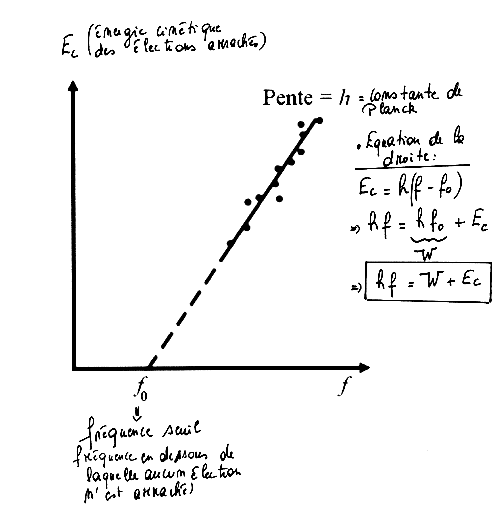
\includegraphics[width=11.102cm,height=11.633cm]{Pictures/10000001000001F0000002085D0C02E9A126192D.png}
\caption{}
\end{figure}

\textbf{Mesure expérimentale de la constante de Planck}

\textbf{(ET DEUX PRIX NOBEL~: EINSTEIN EN 1921 ET PLANCK EN 1923)}



Le physicien américain Millikan apporta la confirmation expérimentale de
l'hypothèse d'Einstein en déterminant pour un même métal, la variation
de l'énergie cinétique des électrons arrachés en fonction de la
fréquence de la lumière monochromatique incidente.

\begin{itemize}

\item
  L'équation de cette droite est bien~:
\end{itemize}

Ec = h(f-f\textsubscript{0})  hf = W + Ec

où h est la pente et a été mesurée expérimentalement~(constante de
Planck) h :

\begin{itemize}

\item
  Chaque métal a une fréquence seuil qui lui est propre.
\end{itemize}

Nous pouvons remarquer sur le graphique que si f = f\textsubscript{0},
alors Ec = 0.

L'énergie du photon incident sera juste suffisante pour arracher
l'électron et ne sera pas suffisante pour encore lui communiquer une
énergie cinétique.

\subsubsection{Comportement quantique de la lumière}

Certains phénomènes (réfraction, diffraction, interférences) ne sont
explicables que par le modèle ondulatoire, d'autres que par le modèle du
photon qui a un comportement corpusculaire.

La lumière se comporte tantôt comme une onde, tantôt comme des
particules.

Finalement, quel est le bon modèle~?

Il est incorrect de dire « la lumière est une onde » ou « la lumière est
une particule ».

En réalité, il n'y a pas de modèle unique pour la lumière.

L'ensemble des comportements de la lumière ne peut s'expliquer ni par
l'un, ni par l'autre des deux modèles. Les deux sont nécessaires, tantôt
c'est l'un qui est efficace, tantôt, c'est l'autre.

\subsubsection{Énergie lumineuse}

Les ondes électromagnétiques transportent de l'énergie, elles sont dites
«~rayonnantes~». C'est la seule forme d'énergie qui peut se propager
dans le vide, en l'absence de matière.

L'énergie lumineuse fait partie des énergies dites « rayonnantes ».

L'énergie lumineuse est proportionnelle au nombre de photons émis (N).

Or chaque photon transporte une énergie qui est proportionnelle à sa
fréquence (E=hf)

Donc, l'énergie lumineuse transportée sera~:

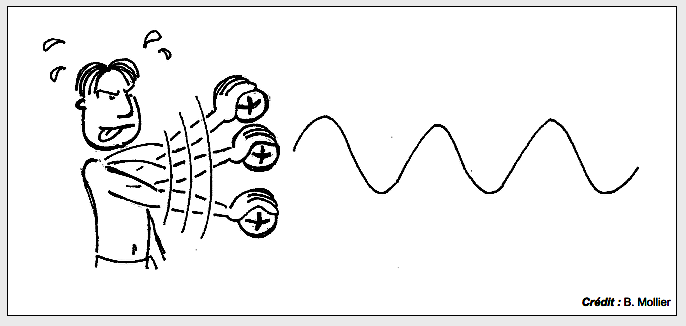
\includegraphics[width=5.433cm,height=2.893cm]{Pictures/10000001000002AE00000146D8BC2B71B32E2C49.png}\emph{\textbf{3
-- QU'EST CE QUE LA LUMIERE~? }

\begin{itemize}

\item
  La lumière est une onde électromagnétique, dont la longueur d'onde,
  comprise entre 400 et 800 nm, correspond à la zone de sensibilité de
  l'œil humain, entre l'ultraviolet et l'infrarouge.
\end{itemize}

\begin{figure}
\centering
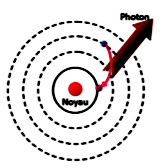
\includegraphics[width=2.847cm,height=2.916cm]{Pictures/10000001000000A4000000A84DE8EBE1FCDB0C87.png}
\caption{}
\end{figure}

\begin{itemize}

\item
  Elle est produite par l'oscillation des électrons atomiques.
\end{itemize}

\begin{itemize}

\item
  Elle constituée d'un ensemble de photons qui sont des quanta d'énergie
  électromagnétique.
\end{itemize}

L'énergie d'un photon dépend de la fréquence.

\begin{itemize}

\item
  L'énergie radiative de la lumière est~:
\end{itemize}

\begin{itemize}

\item
  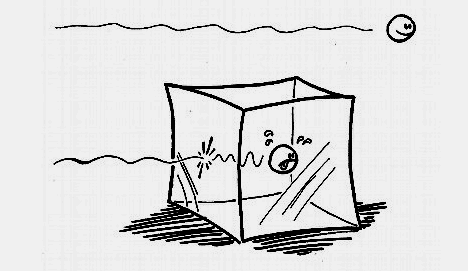
\includegraphics[width=3.861cm,height=2.281cm]{Pictures/10000001000001D40000010F4347AFBBBD12FC87.png}À
  l'inverse des ondes mécaniques (son, vagues,\ldots), la lumière, comme
  toutes les ondes électromagnétiques, n'a pas besoin de support pour se
  propager. Elle peut se déplacer dans le vide et dans un milieu
  transparent (eau, verre,~\ldots).
\end{itemize}

Dans un milieu transparent donc hors du vide, elle se propage moins vite
(cfr. expérience de Young).

On définit l'indice de réfraction du milieu comme étant le rapport de la
vitesse de la lumière dans le vide sur sa vitesse dans le milieu.
(n=c/v)

\begin{itemize}

\item
  La \textbf{lumière est composée} de photons (particules), mais elle
  possède les propriétés d'une onde. Elle a un comportement quantique,
  c'est-à-dire :
\end{itemize}

- La lumière \emph{\textbf{se propage}} \emph{\textbf{comme une onde }}:
elle distribue son énergie dans l'espace de manière continue, comme une
onde. Elle est soumise aux lois de la réflexion, réfraction, diffraction
et interférences.

- La lumière \emph{\textbf{interagit avec la matière de façon discrète}}
: elle échange de l'énergie avec la matière de façon
\textbf{discontinue}, un photon à la fois. L'énergie d'un photon est
proportionnelle à la fréquence.

\subsubsection{Photons et appplications}
% ( Lire p 230 à 236)}
Quelques applications importantes dans la vie quotidienne de l'effet phptoélectrique sont~:
\begin{enumerate}
\item  les cellules photoélectriques
\item  les panneaux photovoltaïques
\item  les diodes LED (pour light emission diod)
\end{enumerate}

\section{Exercices}\label{exercices-photons}


\subsection{Ex. 1}
Une station de radio a une puissance émettrice de 400 kW à 100 MHz.
Combien de photons par seconde sont émis~? (Rép~:
$6.10^{30}$ photons/s)

\subsection{Ex. 2}
Le travail d'extraction d'un électron est de $3,6.10^{-19} \siunits{J}$ pour le potassium.
Soit un faisceau de longueur d'onde égale à 400 nm
qui a une puissance de $10^{-9} \siunits{W}$. Calcule~:
\begin{enumerate}
\item  L'énergie cinétique des électrons émis. $(Rép~:
  1,37.10^{-19} J)$
\item  Le nombre d'électrons émis par mètre carré et par seconde à partir de
  la surface où se produit l'effet photoélectrique, en supposant que 3\%
  des photons incidents parvient à éjecter des électrons. (Rép~:
  $6.10^7$ électrons/s)
\end{enumerate}

\subsection{Ex. 3}
Le seuil photoélectrique de longueur d'onde pour le césium est de 686
nm. Si de la lumière de longueur d'onde égale à 470 nm éclaire la
surface, quelle est la vitesse maximale des électrons émis~? (Rép~:
$5,4.10^5 m/s$)

\subsection{Ex. 4}
Soit un rayonnement de longueur d'onde de 200 nm tombant sur du mercure
pour lequel le travail d'extraction est de 7,2.10\textsuperscript{-19}J.
Quelle est l'énergie cinétique des électrons éjectés~? (Rép~:
$2,74.10^{-19}$ J)

\subsection{Ex. 5}
Lorsqu'un métal est éclairé par de la lumière de fréquence f, l'énergie
cinétique maximale des électrons est de $2,08.10^{-19}$ J.
Lorsqu'on augmente la fréquence de 50\%, l'énergie cinétique maximale
augmente jusqu'à $5,77.10^{-19}$ J.
Quelle est la fréquence seuil de ce métal~? (Rép~: $7,9.10^{14}$ Hz)

\subsection{Ex. 6}

De la lumière bleue (λ = 470 nm) ayant une intensité de 200 W/m² pénètre
dans un œil. Combien de photons entrent dans l'œil par seconde si la
pupille a un diamètre de 5 mm? (Rép~: 9,3.10\textsuperscript{15
}photons/s)

\subsection{Ex. 7}

Lors d'une expérience sur l'effet photoélectrique, on a recueilli les
valeurs suivantes pour la longueur d'onde de la lumière incidente et
l'énergie cinétique des électrons émis

\begin{longtable}[]{@{}llllll@{}}
(nm) & 500 & 450 & 400 & 350 & 300\tabularnewline
Ec (10\textsuperscript{-19} J) & 0,59 & 1,04 & 1,60 & 2,19 &
3,20\tabularnewline
\end{longtable}

Utilise ces données pour calculer \emph{\textbf{graphiquement}} la
valeur de la constante de Planck.

\subsection{Ex. 8}

La longueur d'onde du seuil photoélectrique d'un matériau métallique est
de 360 nm. Quelle est la vitesse maximale des électrons émis si on
utilise des photons de 280 nm de longueur d'onde~? (Rép~:
6.10\textsuperscript{5} m/s)

\subsection{Ex. 9}

De la lumière ayant une longueur d'onde de 450 nm et une intensité de 40
W/m² arrive sur un métal. Combien d'électrons sont éjectés par seconde
et par centimètre carré de surface si seulement 3 \% des photons qui
arrivent sur le métal éjecte un électron?

(Rép~: 2,7.10\textsuperscript{14} électrons/s)

\subsection{Ex. 10}

Lorsqu'un métal est éclairé par de la lumière de fréquence f, l'énergie
cinétique maximale des électrons est de 2,08.10\textsuperscript{-19} J.
Lorsqu'on augmente la fréquence de 50\%, l'énergie cinétique maximale
augmente jusqu'à 5,77.10\textsuperscript{-19} J.

a) Quelle est la fréquence de la source~?
(Rép~:1,1.10\textsuperscript{15} Hz)

b) Sachant que le spectre visible est situé entre 400 nm et 800 nm, la
lumière utilisée est-elle dans le spectre visible, dans la gamme des
ultraviolets ou dans la gamme des infrarouges~? (Rép~: UV)

\subsection{Ex. 11}

Lorsqu'on éclaire une surface avec de la lumière d'une fréquence égale à
7.10\textsuperscript{14 }Hz, les électrons émis ont une vitesse de
5,2.10\textsuperscript{5} m/s. Quelle est la fréquence seuil du métal?

(Rép~: 5,14.10\textsuperscript{14} Hz)

\subsection{Ex. 12}

De la lumière jaune (λ = 585 nm) ayant une intensité de 50 W/m² arrive
sur un mur ayant une surface de 3 m². Combien de photons arrivent sur le
mur en 20 secondes?

(Rép~: 8,8.10\textsuperscript{21} photons/s)

\subsection{Ex. 13}

Les affirmations suivantes sont-elles vraies ou fausses~? Répondre à la
question en indiquant V ou F .

\begin{enumerate}
\item  Lorsqu'on augmente la puissance d'un faisceau laser sans modifier sa
  fréquence, l'effet photoélectrique qu'il produit sur une même surface
  métallique est tel que~:
\item le nombre de photons émis par seconde augmente
\item  l'énergie des photons émis augmente
\item  le nombre d'électrons émis par seconde augmente
\item  l'intensité du courant électrique détecté augmente
\item  l'énergie cinétique des électrons augmente
\end{enumerate}

\subsection{Ex. 14}

Lorsqu'on augmente la fréquence d'un faisceau laser, l'effet
  photoélectrique qu'il produit sur une même surface métallique est tel
  que~:
\begin{enumerate}
  \item    le nombre de photons émis par seconde augmente
  \item    l'énergie des photons émis augmente
  \item le nombre d'électrons émis par seconde augmente
  \item    l'intensité du courant électrique détecté augmente
  \item    l'énergie cinétique des électrons augmente
\end{enumerate}
(Rép~: A) VFVVF, B) FVFVV)

\subsection{Ex. 15}

\begin{enumerate}
\item  Quel est le seuil de longueur d'onde qui permet la photoémission du
  zinc~? Le travail d'extraction du zinc est de
  6,99.10\textsuperscript{-19} J. (Rép~:284 nm)
\item  Cette radiation fait-elle partie du spectre visible de la lumière,
  Justifie. (Rép~: Non)
\item  Quelle sera alors l'énergie cinétique des électrons émis~? Justifie
  (Rép~:1,35.10\textsuperscript{-21} J)
\end{enumerate}

\subsection{Ex. 16}

Un bon niveau d'éclairement pour la lecture correspond à environ
2.10\textsuperscript{13} photons par seconde par centimètre carré. Si
ces photons ont une longueur d'onde moyenne de 500 nm, quelle est
l'intensité lumineuse correspondante~sachant que l'intensité lumineuse
est la puissance reçue par unité de surface.
(Rép~:7,96.10\textsuperscript{-2} W/m\textsuperscript{2})

\subsection{Ex. 17}

Quelle sera la vitesse des électrons émis par du mercure lorsqu'il est
soumis à un rayonnement de longueur d'onde de 200 nm~? Le travail
d'extraction du mercure est de 7,2.10\textsuperscript{-19} J.

(Rép~: 7,8.10\textsuperscript{5} m/s)

\subsection{Ex. 18}

Une station de radio a une puissance émettrice de 400 kW à 100 MHz.
Combien de photons par seconde sont émis~?

\subsection{Ex. 19}

Le travail d'extraction d'un électron est de 3,6.10\textsuperscript{-19}
J pour le potassium. Soit un faisceau de longueur d'onde égale à 400 nm
qui a une puissance de 10\textsuperscript{-9} W. Calcule~:

a) L'énergie cinétique des électrons émis.

b) Le nombre d'électrons émis par mètre carré et par seconde à partir de
la surface où se produit l'effet photoélectrique, en supposant que 3\%
des photons incidents parvient à éjecter des électrons.

\subsection{Ex. 20}

Le seuil photoélectrique de longueur d'onde pour le césium est de 686
nm. Si de la lumière de longueur d'onde égale à 470 nm éclaire la
surface, quelle est la vitesse maximale des électrons émis~?

\subsection{Ex. 21}

Soit un rayonnement de longueur d'onde de 200 nm tombant sur du mercure
pour lequel le travail d'extraction est de 7,2.10\textsuperscript{-19}J.
Quelle est l'énergie cinétique des électrons éjectés~?

\subsection{Ex. 22}

Lorsqu'un métal est éclairé par de la lumière de fréquence f, l'énergie
cinétique maximale des électrons est de 2,08.10\textsuperscript{-19} J.
Lorsqu'on augmente la fréquence de 50\%, l'énergie cinétique maximale
augmente jusqu'à 5,77.10\textsuperscript{-19} J.

Quelle est la fréquence seuil de ce métal~?

\subsection{Ex. 23}

De la lumière bleue (λ = 470 nm) ayant une intensité de 200 W/m² pénètre
dans un œil. Combien de photons entrent dans l'œil par seconde si la
pupille a un diamètre de 5 mm?

\subsection{Ex. 24}

\begin{enumerate}
\item  Lors d'une expérience sur l'effet photoélectrique, on a recueilli les
  valeurs suivantes pour la longueur d'onde de la lumière incidente et
  l'énergie cinétique des électrons émis
\end{enumerate}

\begin{longtable}[]{@{}llllll@{}}
(nm) & 500 & 450 & 400 & 350 & 300\tabularnewline
$E_c$ ($10^{-19}$ J) & 0,59 & 1,04 & 1,60 & 2,19 &
3,20\tabularnewline
\end{longtable}

Utilise ces données pour calculer \emph{graphiquement} la
valeur de la constante de Planck.

\subsection{Ex. 25}

La longueur d'onde du seuil photoélectrique d'un matériau métallique est
de 360 nm. Quelle est la vitesse maximale des électrons émis si on
utilise des photons de 280 nm de longueur d'onde~?

\subsection{Ex. 26}

De la lumière ayant une longueur d'onde de 450 nm et une intensité de 40
W/m² arrive sur un métal. Combien d'électrons sont éjectés par seconde
et par centimètre carré de surface si seulement 3 \% des photons qui
arrivent sur le métal éjecte un électron?

\subsection{Ex. 27}

Lorsqu'un métal est éclairé par de la lumière de fréquence f, l'énergie
cinétique maximale des électrons est de 2,08.10\textsuperscript{-19} J.
Lorsqu'on augmente la fréquence de 50\%, l'énergie cinétique maximale
augmente jusqu'à 5,77.10\textsuperscript{-19} J.

a) Quelle est la fréquence de la source~?

b) Sachant que le spectre visible est situé entre 400 nm et 800 nm, la
lumière utilisée est-elle dans le spectre visible, dans la gamme des
ultraviolets ou dans la gamme des infrarouges~?

\subsection{Ex. 28}

Lorsqu'on éclaire une surface avec de la lumière d'une fréquence égale à
7.10\textsuperscript{14 }Hz, les électrons émis ont une vitesse de
5,2.10\textsuperscript{5} m/s. Quelle est la fréquence seuil du métal?

\subsection{Ex. 29}

De la lumière jaune (λ = 585 nm) ayant une intensité de 50 W/m² arrive
sur un mur ayant une surface de 3 m². Combien de photons arrivent sur le
mur en 20 secondes?

\subsection{Ex. 30}

Les affirmations suivantes sont-elles vraies ou fausses~? Répondre à la
question en indiquant V ou F .

A) Lorsqu'on augmente la puissance d'un faisceau laser sans modifier sa
fréquence, l'effet photoélectrique qu'il produit sur une même surface
métallique est tel que~:
\begin{enumerate}
\item  le nombre de photons émis par seconde augmente
\item  l'énergie des photons émis augmente
\item  le nombre d'électrons émis par seconde augmente
\item  l'intensité du courant électrique détecté augmente
\item  l'énergie cinétique des électrons augmente
\end{enumerate}

B) Lorsqu'on augmente la fréquence d'un faisceau laser, l'effet
photoélectrique qu'il produit sur une même surface métallique est tel
que~:
\begin{enumerate}
  \item    le nombre de photons émis par seconde augmente
  \item    l'énergie des photons émis augmente
  \item  le nombre d'électrons émis par seconde augmente
  \item    l'intensité du courant électrique détecté augmente
  \item    l'énergie cinétique des électrons augmente
\end{enumerate}

\subsection{Ex. 31}

\begin{enumerate}
\item  Quel est le seuil de longueur d'onde qui permet la photoémission du
  zinc~? Le travail d'extraction du zinc est de
  6,99.10\textsuperscript{-19} J.
\item  Cette radiation fait-elle partie du spectre visible de la lumière,
  Justifie.
\item  Quelle sera alors l'énergie cinétique des électrons émis~? Justifie
\end{enumerate}

\subsection{Ex. 32}

Un bon niveau d'éclairement pour la lecture correspond à environ
$2 \quad 10^{13}$ photons par seconde par centimètre carré. Si
ces photons ont une longueur d'onde moyenne de 500 nm, quelle est
l'intensité lumineuse correspondante~sachant que l'intensité lumineuse
est la puissance reçue par unité de surface.

\subsection{Ex. 33}

Quelle sera la vitesse des électrons émis par du mercure lorsqu'il est
soumis à un rayonnement de longueur d'onde de 200 nm~? Le travail
d'extraction du mercure est de 7,2.10\textsuperscript{-19} J.

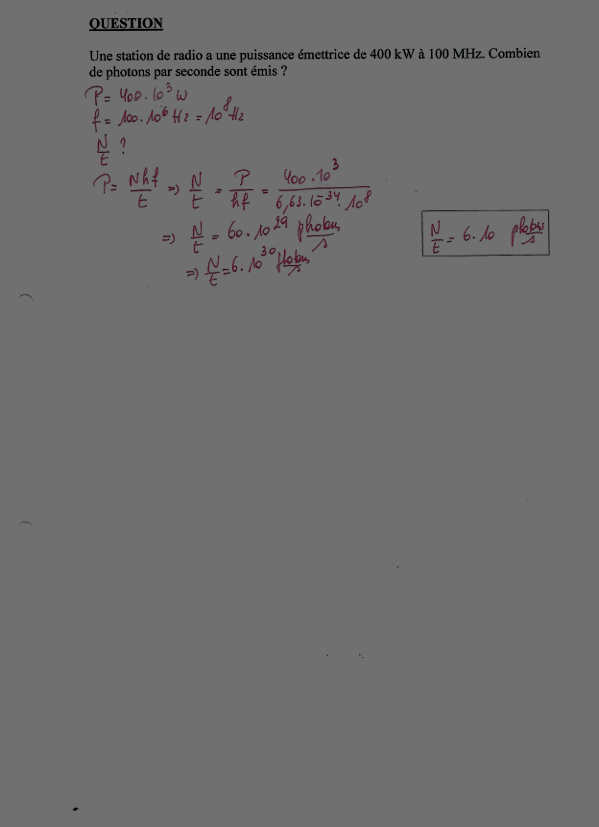
\includegraphics[width=17.448cm,height=24.063cm]{Pictures/10000001000002570000033B23A9DDE6A8AAA6C6.png}

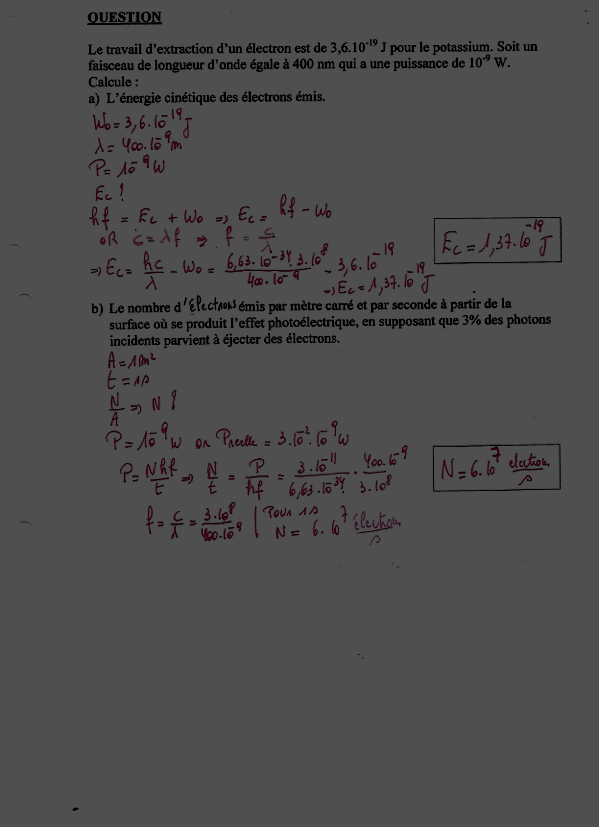
\includegraphics[width=17.498cm,height=24.13cm]{Pictures/10000001000002570000033B4A6387CB4865E463.png}

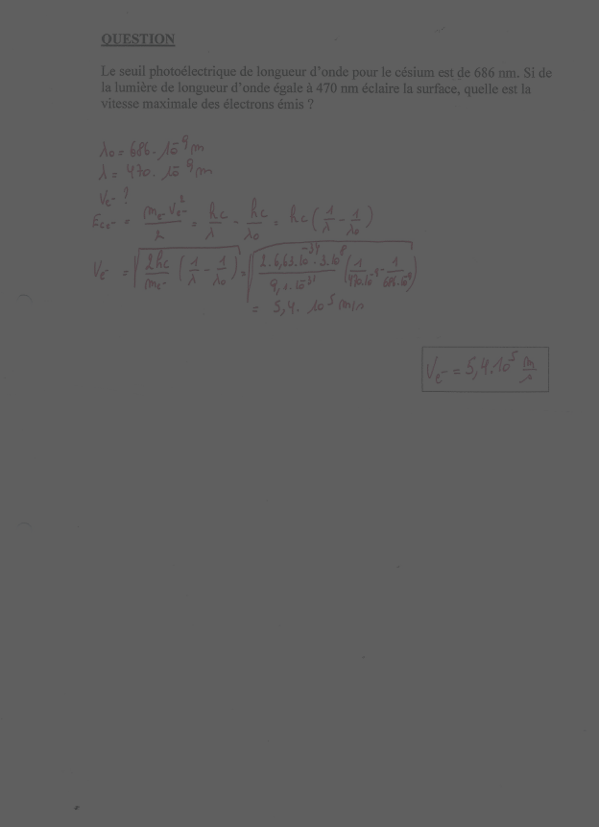
\includegraphics[width=17.498cm,height=24.13cm]{Pictures/10000001000002570000033B5842099DBC063D07.png}


\includegraphics[width=17.498cm,height=24.13cm]{Pictures/10000001000002570000033B2EDAF7105EA9C179.png}


\includegraphics[width=17.498cm,height=24.13cm]{Pictures/10000001000002570000033B637F3053717E0CEA.png}

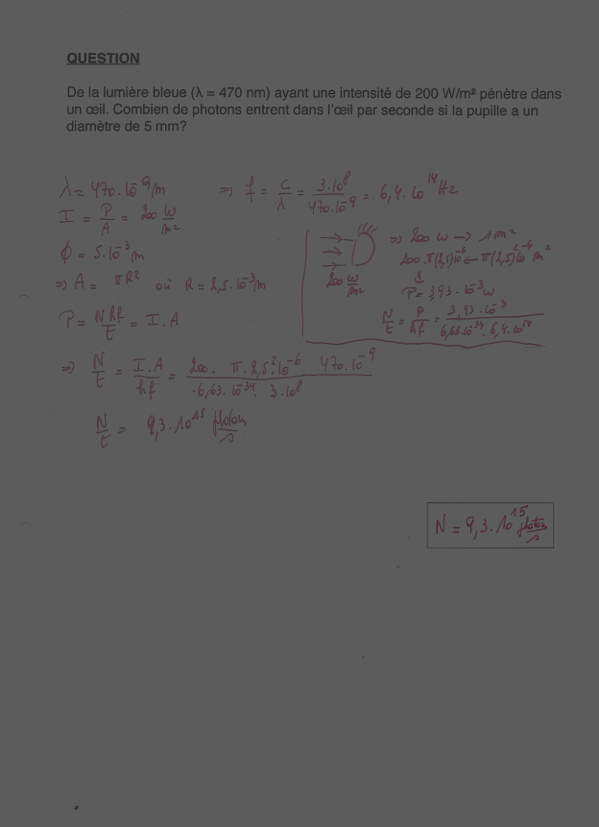
\includegraphics[width=17.498cm,height=24.13cm]{Pictures/10000001000002570000033B1D8D222AA0515BC3.png}


\includegraphics[width=17.498cm,height=24.13cm]{Pictures/10000001000002570000033BD2AA64816C97C97B.png}


\includegraphics[width=17.498cm,height=24.13cm]{Pictures/10000001000002570000033B115B7FCA5E9F77EB.png}


\includegraphics[width=17.498cm,height=24.13cm]{Pictures/10000001000002570000033B834634AAD14CB84E.png}

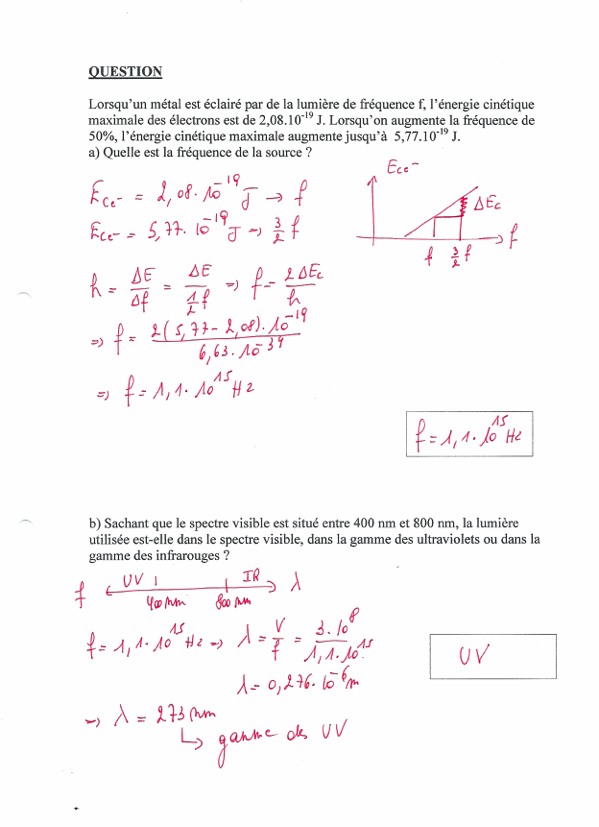
\includegraphics[width=17.498cm,height=24.13cm]{Pictures/10000001000002570000033BF05D77DDF7E1650A.png}

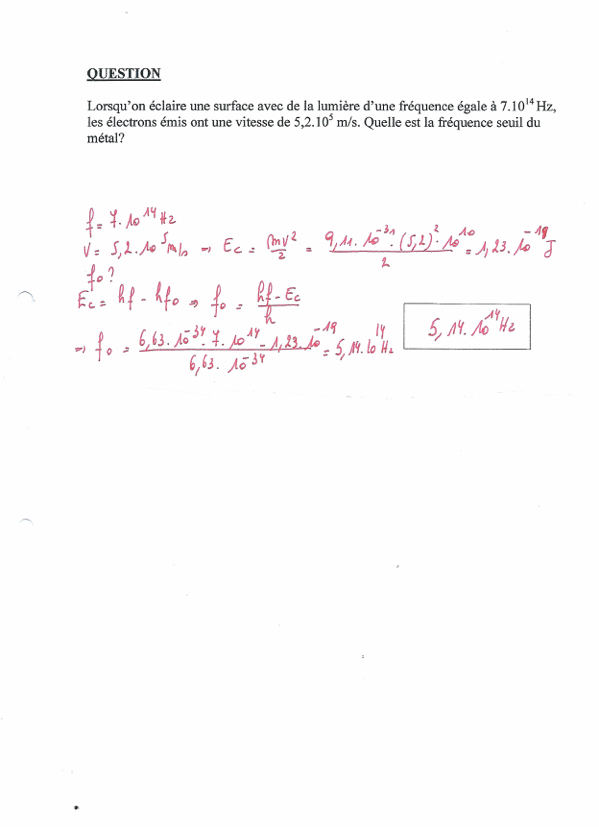
\includegraphics[width=17.498cm,height=24.13cm]{Pictures/10000001000002570000033B282FC06DC4D6D42C.png}

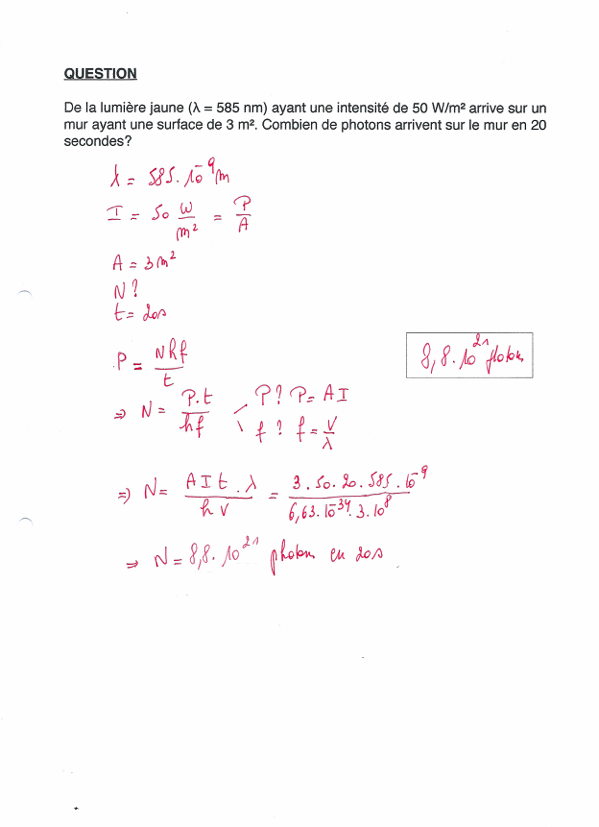
\includegraphics[width=17.498cm,height=24.13cm]{Pictures/10000001000002570000033B9D23F92FA4FE8FB5.png}

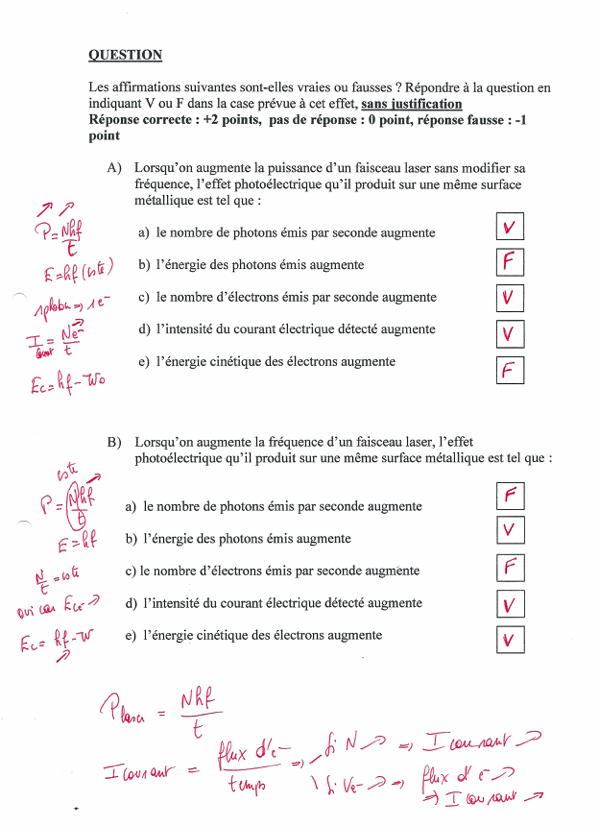
\includegraphics[width=17.498cm,height=24.13cm]{Pictures/10000001000002570000033B70807DBABEAE0DEC.png}

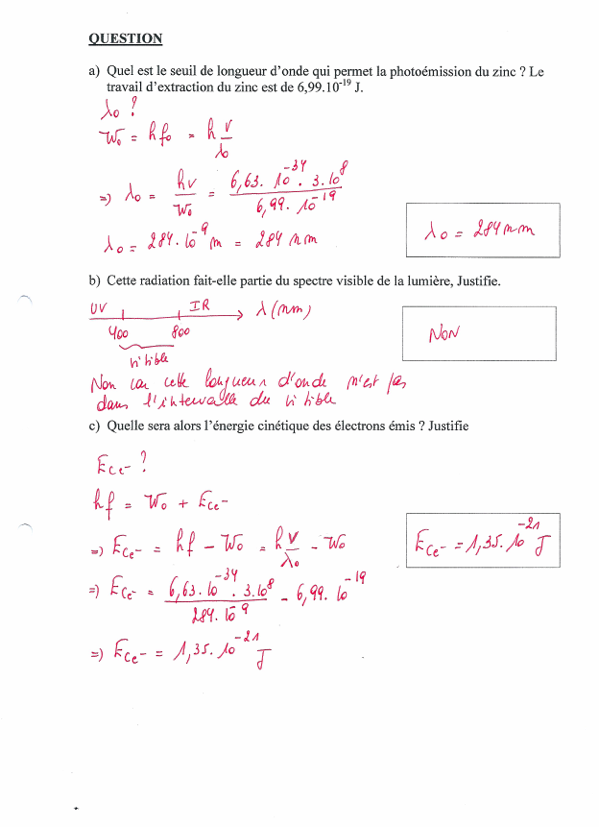
\includegraphics[width=17.498cm,height=24.13cm]{Pictures/10000001000002570000033BB37256DDDEE8E8E4.png}

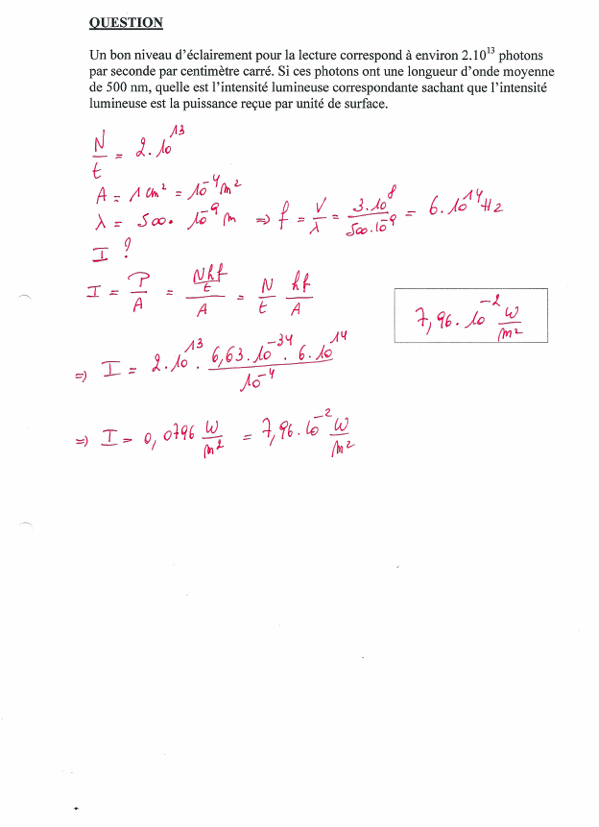
\includegraphics[width=17.498cm,height=24.13cm]{Pictures/10000001000002570000033BCFBA7D32EF4FFF20.png}

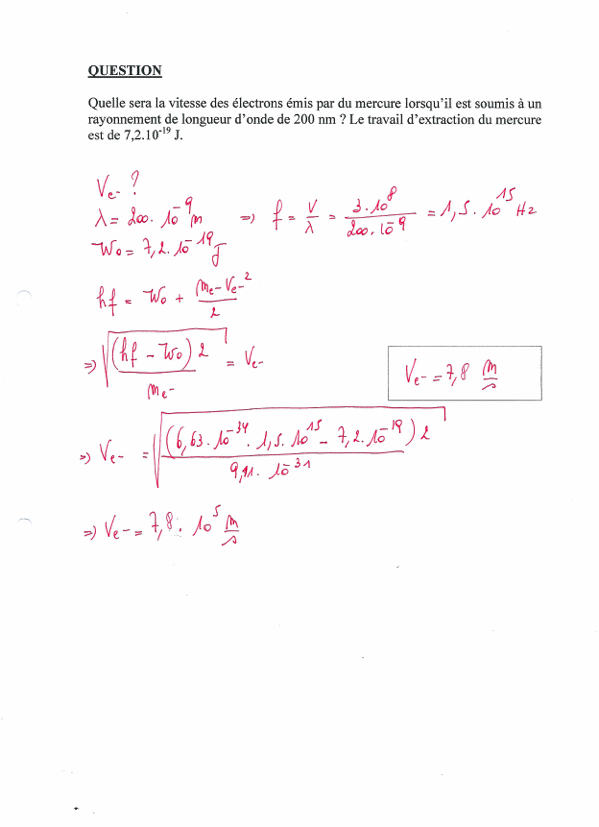
\includegraphics[width=17.498cm,height=24.13cm]{Pictures/10000001000002570000033B7F417BAE8163DC5F.png}
